\chapter{Lab work} 
\pagenumbering{arabic}
\label{chap_Intro}

In this lab we create a group management system where multiple nodes are connected and they all keep the same state. All messages are always sent to all connected nodes as the state depends on all previously received messages. To illustrate their behaviour we create graphical windows with a colour depending on all previously received messages. In figure \ref{fig:diagram} we illustrate the overall structure of the system.

\begin{figure}[h]
\centering
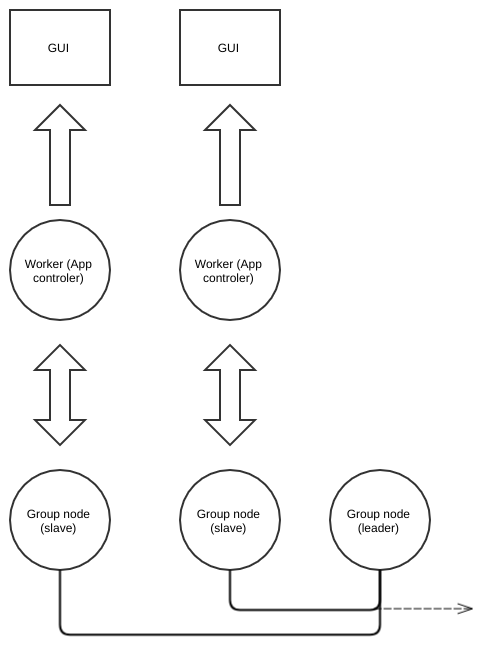
\includegraphics[width=0.5\linewidth]{res/diagram}
\caption{System structure}
\label{fig:diagram}
\end{figure}

The lab work mainly focuses on creating the logic of the group service and code for the Application and GUI was provided and only extended in functionality by adding this new module for group synchronization. The group nodes (which all lives in separate erlang processes) can be either a slave or a leader node which perform their task a bit different. The slave nodes always sends messages to the leader when trying to broadcast a change to the entire group. The leader node on the other hand will instead receive broadcast requests and send out messages to all the slaves in the network. This makes sure that all messages are received in the same order by all nodes as it is a single process that is sending them all and erlang guarantees a FIFO order of messages between processes.

One problem here is that the leader node can die which means that the other nodes no longer have any way to communicate. To solve this we use the built in feature where we can monitor a process and receive a message if it dies. All processes therefore monitor their leader and take action if something happens to it. The slave processes will then always choose the first process in the list of nodes in the network and select it as the new leader. As all nodes have the same list which represent the network, this means that all nodes will choose the same leader (otherwise we have a problem). 

In case a leader dies while it is broadcasting messages to the nodes in the network we might have a situation where some nodes never receives the message currently being broadcasted. To solve this problem all nodes keep track of the last seen message and the leader node will broadcast that to the network when a leader dies. To prevent nodes from receiving the same message twice (which they often will do with this implementation) we add a sequence number to all messages. This way all nodes can discard messages they have already received.

\section{Problems and further development}
One problem with the current implementation is that it will not account for lost messages. Erlang will guarantee FIFO order of messages between two processes but does not guarantee that messages are delivered. This means that we can loose a message to one of the slave nodes and that process will thereafter be out of sync compared to the rest of the network. To solve this we have two primary options. We can either store all messages in a list until we are certain that all nodes has received them (and using acknowledgements when nodes receive messages). Or we can have the leader node wait for all nodes to acknowledge each message it sends before moving on to handling more messages. In the second implementation we are not required to store as much data and problems where the leader node crashes are simpler to solve. The network will also become more synchronized with this implementation as only one message will ever be sent before all nodes has to synchronize again. On the other side this way of solving the problem has a lot of performance issues. The entire system will lock down if a single node fails to respond and we have to wait for it to time out or answer. This means that we can no longer toggle state faster than the maximum round trip time in the system which we could do previously.